\chapter{範例 はんれい}\label{example}

% 表格範例
\section{表格}
\begin{table}[h]
   \centering
   \caption{tabular 表格的基本結構}\label{booktabs_1}
		\begin{tabular}[t]{lll}
		\hline
		column1 & column2 & column3 \\
		\hline
		item1   & item2   & item3 \\
		itemA   & itemB   & itemC \\
		\hline
		\end{tabular}
\end{table}
\clearpage

\subsection{對齊小數點}
\begin{tabular}{lD{.}{.}{3}D{.}{.}{3}D{.}{.}{3}D{.}{.}{3}}
   \toprule
         & headA & headB & headC & headD \\
   \midrule
   test1 & 65536  & 32768 & 1382.81 & 998.98 \\
   test2 & 12.457 & 35.21 & 321.3   & 51787.787 \\
   test3 & 211.97 & 5.2457& 23.6449 & 74294.106 \\
   \bottomrule
\end{tabular}
\clearpage

\begin{landscape}
    \begin{table}[h]
    \caption{橫著放}
    \label{Tab:Commercial_App_Features_Comparison}
    \begin{center}               
    \begin{tabular}{|c|c|c|c|c|c|c|c|c|}
    \hline
       & column1  & column2  & column3 & column4 & column5 & column6 & column7 & column8 \\ \hline
    1. & item1    & -        & -       & -       & -       &     \color{red}{${\surd}$} &  \color{red}{${\surd}$}    &  \color{red}{${\surd}$}     \\ \hline
    2. & item2    & -        & -       & -       & \color{red}{${\surd}$}      & \color{red}{${\surd}$}     & -    & -     \\ \hline
    3. & item3    & -        & -       & \color{red}{${\surd}$} & -     &  -    &  \color{red}{${\surd}$}    & -     \\ \hline
    4. & item4    & -        & -       & -       &  \color{red}{${\surd}$}     &  -    & -    &      \color{red}{${\surd}$} \\ \hline
    5. & item5    & -        & -       & -       &  -   &    \color{red}{${\surd}$}  &  \color{red}{${\surd}$}    &  \color{red}{${\surd}$}     \\ \hline
    6. & item6    & -        & -       & -       &  \color{red}{${\surd}$}   &  -    & -    &      - \\ \hline
    7. & item7    & -        & -       & -       &  -     &  \color{red}{${\surd}$}    & -    &     *- \\ \hline
    8. & item8    & -        & -       & -       &   \color{red}{${\surd}$}    &   \color{red}{${\surd}$}   & -    &      \color{red}{${\surd}$} \\ \hline
    9. & item9    &  \color{red}{${\surd}$}    &  -    & \color{red}{${\surd}$}                  &   \color{red}{${\surd}$}    &   \color{red}{${\surd}$}   &  \color{red}{${\surd}$}    &  \color{red}{${\surd}$}     \\ \hline
    \end{tabular}
    \end{center}
    \end{table}
 \end{landscape}
 \clearpage

 % 圖片範例
 \section{插入圖片}
 \LaTeX 圖片插入範例區塊。

\subsection{插圖範例}
\begin{figure}[h]
圖片插入範例: \\
   \centering
   
\includegraphics[width=10cm]{../Figures/Result/我就爛}
   \caption{我就爛}\label{fig:我就爛}

   \subfigure[你也爛]{
      
\includegraphics[width=5cm]{../Figures/Result/你也爛}
      \hspace{0.5 in}
   }
   \subfigure[一起爛]{
      
\includegraphics[width=5cm]{../Figures/Result/一起爛}
   }
   \caption{爛起來}\label{fig:爛起來}
\end{figure}
圖片插入及圖片並排測試。
\clearpage

% 繪圖範例
\subsection{繪圖範例}
\begin{figure}[h]
繪圖範例 1: \\
   \centering
      \pgfplotsset{width=10cm}         % 設置繪圖尺寸
      \begin{tikzpicture}
         \begin{axis}                  % 繪製座標
            % dashes = [10, 5, 100, 5] # 10 points on, 0 off, 100 on, 0 off
            \addplot [dash pattern=on 10 off 0 on 100 off 0, domain=0:6, samples=100, very thick, cyan] {sin(deg(x))};
         \end{axis}
      \end{tikzpicture}
   \caption{SIN FUNCTION}\label{fig:SIN FUNCTION}
\end{figure}
正弦波形繪製

繪圖範例2:
\begin{center}
    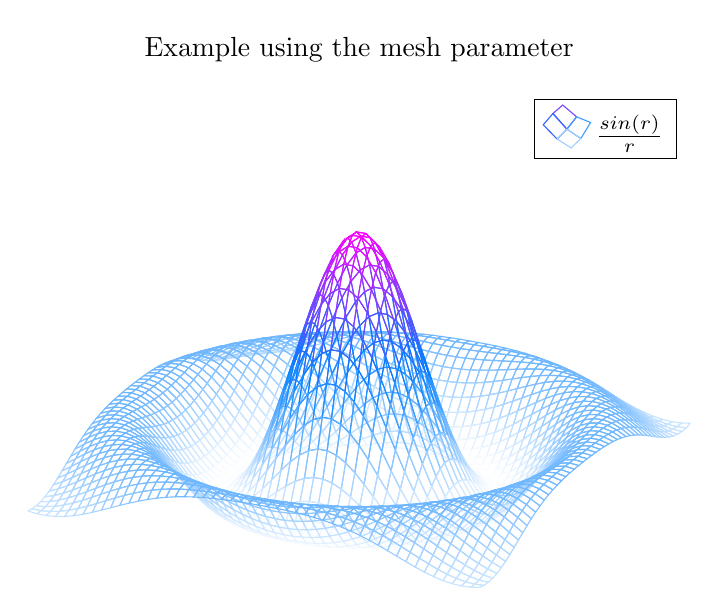
\begin{tikzpicture}
        \begin{axis}[
            title=Example using the mesh parameter, % 圖標題
            hide axis,                              % 隱藏座標
            colormap/cool,                          % 顏色風格
        ]
        \addplot3[
            mesh,                                   % 繪製的三維圖像是網格
            samples=50,                             % 定義域分割數量
            domain=-8:8,                            % 定義域
        ]
        {sin(deg(sqrt(x^2+y^2)))/sqrt(x^2+y^2)};    % 二元顯式函數
        \addlegendentry{$\frac{sin(r)}{r}$}         % 添加圖例
        \end{axis}
        \end{tikzpicture}
\bfseries
\end{center}

% 公式範例
\section{公式}
\begin{equation}
   \sqrt[n]{\frac{x^2+\sqrt 2}{x+y}}
\end{equation}

\begin{equation}
   a:b:c = ma : mb: mc = \frac{a}{m} : \frac{b}{m} : \frac{c}{m} , (m \neq 0)
\end{equation}

\begin{equation}
\lim_{n \to \infty}\sum_{i=1}^n{\frac{1}{n}}\sin\frac{k}{n}
\end{equation}

\begin{equation}
   g(x,y) = \left\{\begin{array}{ll}
      f(x,y), & \mbox{if $x<y$} \\  % 文字的部份要用 \mbox
      f(y,x), & \mbox{if $x>y$} \\  % 包住,讓他使用正常字體
      0,      & \mbox{otherwise.}
     \end{array} \right.
\end{equation}

\begin{equation}
   A =\begin{pmatrix}                % 使用小括號
  t_{11} & t_{12} & t_{13} \\
  t_{21} & t_{22} & t_{23} \\
  t_{31} & t_{32} & t_{33}
   \end{pmatrix}
\end{equation}
\vspace*{3em}

歐姆定律(Ohm's law),如式\ref{eq_ohm_v}所示,$V$是電壓,$I$是電流,比例常數$R$是電阻。

\begin{equation}\label{eq_ohm_v}
    \begin{split}
        V = I \cdot R
    \end{split}
\end{equation}
\clearpage

% 註腳範例
\section{利用註腳,收納資料}
腳註,又名註腳、筆記、札記(德語:Fußnote;英語:Footnote),是讀書所做的筆錄、見解、體會、看法、觀點、心得、感想的總稱。
腳註分為:頭注、側注、後注、割注、分注。
\footnote{腳註的格式有時候是零散的、即興的、偶然的、信筆成文的,因此它並不是有章法的、系統的、全面的、學術論文式樣的行筆條理清晰。腳註不同於參考文獻(交互參照),有對於原文若干字句、詞語、典故、暗示、比喻等文筆的疏通和講解。}
在版面的下方,\LaTeX 會畫一條短線,用比較小的字型將附註的編號和內容安排在短線之下。


% 字體範例
\section{字體}
\subsection{文字特效}
中文文字特效, Hello world!\\
{\LARGE
\textbf{Hello world!, bold face, 粗體} \\
\textit{Hello world!, italic, 斜體} \\
\textsl{Hello world!, slanted, 傾斜} \\
\underline{Hello world!, underline, 底線} \\
}

英文文字家族,Hello world!\\
{\LARGE
\textrm{Hello world!, roman, 羅馬} \\
\texttt{Hello world!, typewriter, 等寬} \\
\textsf{Hello world!, sans serif} \\
\textsc{Hello world!, Small Caps} \\
}

% 文字範例
\section{文字大小}
一般文字大小範例, Font Size.\\
{\tiny 文字大小範例, Font Size.}\\
{\scriptsize 文字大小範例, Font Size.}\\
{\footnotesize 文字大小範例, Font Size.}\\
{\small 文字大小範例, Font Size.}\\
{\normalsize 文字大小範例, Font Size.}\\
{\large 文字大小範例, Font Size.}\\
{\Large 文字大小範例, Font Size.}\\
{\LARGE 文字大小範例, Font Size.}\\
{\huge 文字大小範例, Font Size.} \\
{\Huge 文字大小範例, Font Size.}
\clearpage

\section{醒目提示範例}
\colorbox{yellow}{黃底黑字。} \\
\color{blue}{青い文字} \\
\color{red}{\colorbox{pink}{Red color box and red font.}} \\
\color{black}{最後請記得回復成預設黑色字體}

\subsection{盒子}
Latex排板小到一個字母,大到一個段落,都可以視為一個矩型盒子(box),就像html一樣。

mbox:
\mbox{只是一個句子 被組合成盒子 的句子}

fbox:
\fbox{只是一個句子 被組合成盒子 但是有外框 的句子}

makebox/framebox:可加上一些設定的盒子

%語法:[寬][對齊]{內容}
\makebox[\textwidth][c]{只是一個句子 被組合成盒子 的句子}

\framebox[0.5\textwidth][r]{被組合成盒子 但是有外框 的句子 還不夠寬}

\newpage

